\usetikzlibrary{calc,trees,positioning,arrows,chains,shapes.geometric,%
    decorations.pathreplacing,decorations.pathmorphing,shapes,%
    matrix,shapes.symbols}

\tikzset{
>=stealth',
  punktchain/.style={
    rectangle, 
    rounded corners, 
    % fill=black!10,
    draw=black, very thick,
    text width=22em, 
    minimum height=3em, 
    text centered, 
    on chain},
  line/.style={draw, thick, <-},
  element/.style={
    tape,
    top color=white,
    bottom color=blue!50!black!60!,
    minimum width=8em,
    draw=blue!40!black!90, very thick,
    text width=10em, 
    minimum height=3.5em, 
    text centered, 
    on chain},
  every join/.style={->, thick,shorten >=1pt},
  decoration={brace},
  tuborg/.style={decorate},
  tubnode/.style={midway, right=2pt},
}
\begin{figure}[htb]
\small
  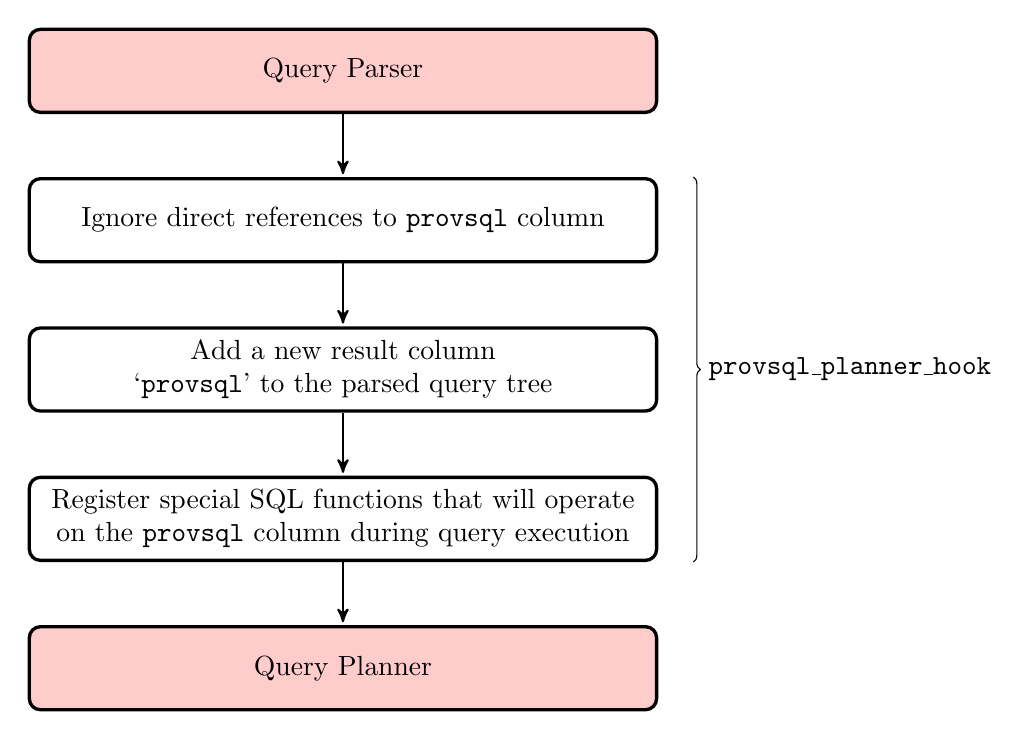
\begin{tikzpicture}
  [node distance=.8cm,
  start chain=going below,]
    %  \node[punktchain, fill=yellow!20] (input) {Input query};
     \node[punktchain, join, fill=red!20] (parser) {Query Parser};
     \node[punktchain, join] (A) {Ignore direct references to \texttt{provsql} column};
     \node[punktchain, join] (B) {Add a new result column `\texttt{provsql}' to the parsed query tree};
     \node[punktchain, join] (C) {Register special SQL functions that will operate on the \texttt{provsql} column during query execution};
    \node[punktchain, join, fill=red!20] (planner) {Query Planner};
    % \node[punktchain, join, fill=green!20] (output) {Query result:\\ includes a \texttt{provsql} column of tokens, identifying gates of the prov. circuit};
  % Now that we have finished the main figure let us add some "after-drawings"
  % Now, let us add some braches. 
  %% No. 1
%   \draw[tuborg, decoration={brace}] let \p1=(init.north), \p2=(init.south) in
%     ($(2, \y1)$) -- ($(2, \y2)$) node[tubnode] {Called once, upon extension loading};
%   %% No. 2
%   \draw[tuborg, decoration={brace}] let \p1=(fini.north), \p2=(fini.south) in
%     ($(2, \y1)$) -- ($(2, \y2)$) node[tubnode] {Called once, upon extension unloading};
  %% No. 3
  \draw[tuborg, decoration={brace}] let \p1=(A.north), \p2=(C.south) in
    ($(4.45, \y1)$) -- ($(4.45, \y2)$) node[tubnode] {\texttt{provsql\_planner\_hook}};
  \end{tikzpicture}
   \textbf{\caption{\label{fig:provsql_architecture}ProvSQL system architecture.}}
\normalsize
\end{figure}
%%% Local Variables: 
%%% mode: latex
%%% TeX-master: t
%%% End: